\documentclass{article}
\usepackage{subcaption}
\usepackage{graphicx}
\usepackage{multicol} % Allows for multiple columns
\usepackage[squaren,Gray]{SIunits}
\usepackage{multirow}
\usepackage{makecell}
\usepackage[compat=1.1.0]{tikz-feynman}
\usepackage[textsize=tiny,backgroundcolor=white]{todonotes}
\usepackage[top=1in, bottom=1.25in, left=0.8in, right=0.8in]{geometry}
\begin{document}
        \begin{center}
    {\LARGE \bf Generating Feynman Diagrams}
\end{center}

\vspace{3cm}
{\Large \bf Color Scheme:}
\begin{center}
    \begin{itemize}
        \item {\begin{tikzpicture}[baseline= (base)]
    \begin{feynman}
        \vertex (a);
        \vertex[right=2.8cm of a] (b);
        
    \diagram*{
    (a)--[fermion, color=red] (b),
    };
    \end{feynman}
    \coordinate [yshift=-2.5pt] (base) at (b);
\end{tikzpicture} \hspace{1cm} Up ($U$) quark}
   \item {\begin{tikzpicture}[baseline= (base)]
    \begin{feynman}
        \vertex (a);
        \vertex[right=2.8cm of a] (b);
        
    \diagram*{
    (a)--[fermion, color=violet] (b),
    };
    \end{feynman}
    \coordinate [yshift=-2.5pt] (base) at (b);
\end{tikzpicture} \hspace{1cm} anti-Up ($\overline{U}$) quark}

   \item {\begin{tikzpicture}[baseline= (base)]
    \begin{feynman}
        \vertex (a);
        \vertex[right=2.8cm of a] (b);
        
    \diagram*{
    (a)--[fermion, color=purple] (b),
    };
    \end{feynman}
    \coordinate [yshift=-2.5pt] (base) at (b);
\end{tikzpicture} \hspace{1cm} Down ($D$) quark}

   \item {\begin{tikzpicture}[baseline= (base)]
    \begin{feynman}
        \vertex (a);
        \vertex[right=2.8cm of a] (b);
        
    \diagram*{
    (a)--[fermion, color=orange] (b),
    };
    \end{feynman}
    \coordinate [yshift=-2.5pt] (base) at (b);
\end{tikzpicture} \hspace{1cm} anti-Down ($\overline{D}$) quark}

   \item {
\begin{tikzpicture}[baseline= (base)]
    \begin{feynman}
        \vertex (a);
        \vertex[right=2.8cm of a] (b);
        
    \diagram*{
    (a)--[gluon, color=green] (b),
    };
    \end{feynman}
    \coordinate [yshift=-2.5pt] (base) at (b);
\end{tikzpicture} \hspace{1cm} Gluon $(g)$}

   \item {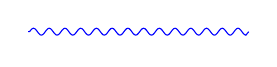
\begin{tikzpicture}[baseline= (base)]
    \begin{feynman}
        \vertex (a);
        \vertex[right=2.8cm of a] (b);
        
    \diagram*{
    (a)--[boson, color=blue] (b),
    };
    \end{feynman}
    \coordinate [yshift=-2.5pt] (base) at (b);
\end{tikzpicture} \hspace{1cm} $Z$ boson}

   \item {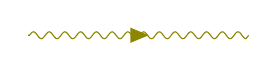
\begin{tikzpicture}[baseline= (base)]
    \begin{feynman}
        \vertex (a);
        \vertex[right=2.8cm of a] (b);
        
    \diagram*{
    (a)--[charged boson, color=olive] (b),
    };
    \end{feynman}
    \coordinate [yshift=-2.5pt] (base) at (b);
\end{tikzpicture} \hspace{1cm} $W^+$ boson}

   \item {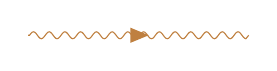
\begin{tikzpicture}[baseline= (base)]
    \begin{feynman}
        \vertex (a);
        \vertex[right=2.8cm of a] (b);
        
    \diagram*{
    (a)--[charged boson, color=brown] (b),
    };
    \end{feynman}
    \coordinate [yshift=-2.5pt] (base) at (b);
\end{tikzpicture} \hspace{1cm} $W^-$ boson}

   \item {\begin{tikzpicture}[baseline= (base)]
    \begin{feynman}
        \vertex (a);
        \vertex[right=2.8cm of a] (b);
        
    \diagram*{
    (a)--[ghost, color=yellow] (b),
    };
    \end{feynman}
    \coordinate [yshift=-2.5pt] (base) at (b);
\end{tikzpicture} \hspace{1cm} Ghosts ($gh$)}

   \item {
\begin{tikzpicture}[baseline= (base)]
    \begin{feynman}
        \vertex (a);
        \vertex[right=2.8cm of a] (b);
        
    \diagram*{
    (a)--[boson, color=teal] (b),
    };
    \end{feynman}
    \coordinate [yshift=-2.5pt] (base) at (b);
\end{tikzpicture} \hspace{1cm} Vector ($V$) boson, and Photon ($\gamma$)}
    \end{itemize}
\end{center}
\newpage


\include{d3l}

\end{document}
